En este capítulo se describe el desarrollo del código desarrollado, desde la primera versión del juego Snake hasta la versión final. Se explican los principales problemas encontrados y las soluciones propuestas para resolverlos. Además, se detallan las principales funciones y estructuras de datos utilizadas en el código.

\section{Version 1: Snake en C++ para ordenadores de escritorio}

La primera versión del juego Snake se desarrolló en C++ utilizando la librería estándar de C++ (STL). El objetivo de esta versión era crear un juego funcional que pudiera ser ejecutado en ordenadores de escritorio. El código se desarrolló en Visual Studio Code, que ofrece una interfaz gráfica intuitiva para escribir, compilar, depurar y ejecutar código C++.

\subsection{Estructura del código}

El código se divide en la siguiente estructura de carpetas:

\begin{itemize}
\item \textbf{src}: contiene los archivos de código fuente. Dónde se implementan las funciones.
\item \textbf{include}: contiene los archivos de cabecera. Dónde se declaran las funciones y variables.
\item \textbf{bin}: contiene los archivos ejecutables.
\end{itemize}


\subsection{Clases y estructuras de datos}

El código se divide en las siguientes clases y estructuras de datos:

\subsubsection{Clase \texttt{Board}}

La clase \texttt{Board} representa el tablero de juego en la implementación del juego Snake. Esta clase es fundamental para gestionar la lógica del juego, incluyendo el estado del tablero, la posición y movimiento de la serpiente, y la generación de alimentos.

Atributos y Métodos:

\begin{itemize}
    \item \textbf{Enumeración Square:} Define los posibles estados de cada cuadrado del tablero: vacío, comida, cuerpo de la serpiente y cabeza de la serpiente.
    \item \textbf{Constructores y Destructor:} La clase proporciona constructores para inicializar el tablero con dimensiones específicas y un destructor para la gestión adecuada de recursos.
    \item \textbf{Getters:} Métodos para obtener información sobre el tablero, como su ancho, alto y el estado de los cuadrados.
    \item \textbf{Métodos de Verificación:} Incluye funciones para verificar si una posición específica en el tablero corresponde a un borde, comida, cuerpo o cabeza de la serpiente.
    \item \textbf{turnGame y moveSnake:} Métodos para manejar el turno del juego y el movimiento de la serpiente, respectivamente.
    \item \textbf{Generación y Consumo de Comida:} Métodos para generar comida en el tablero y manejar su consumo por parte de la serpiente. La generación de comida se realiza de forma aleatoria y asegurando que no se genere en la posición actual de la serpiente.
    \item \textbf{gameOver:} Método para manejar el fin del juego.
    \item \textbf{Sobrecarga de Operadores:} Sobrecarga del operador de índice para acceder a los estados de los cuadrados del tablero y del operador de inserción para imprimir el tablero.
    \item \textbf{displayBoard:} Método para mostrar el tablero en un gestor de visualización.
\end{itemize}

Estructura Interna: 

\begin{itemize}
    \item \textbf{Atributos Privados:} Incluyen dimensiones del tablero, un puntero a un vector de vectores representando el estado de cada cuadrado, y un puntero a la instancia de la serpiente.
    \item \textbf{Métodos Privados:} Métodos para cambiar el estado de los cuadrados del tablero en respuesta a los movimientos de la serpiente.
\end{itemize}

Funcionalidad:

La clase \texttt{Board} actúa como el núcleo lógico del juego, manteniendo el estado del tablero y respondiendo a las interacciones del jugador y a los cambios en el juego. Su diseño modular y su conjunto de métodos bien definidos facilitan la gestión del estado del juego y la interacción con otros componentes, como la serpiente y el sistema de visualización.


\subsubsection{Clase \texttt{Snake}}

La clase \texttt{Snake} es responsable de representar y gestionar la serpiente en el juego. Esta clase controla el movimiento, el crecimiento y las interacciones de la serpiente con otros elementos del juego como la comida y los límites del tablero.

Atributos y Métodos:

\begin{itemize}
    \item \textbf{Constructores y Destructor:} La clase \texttt{Snake} proporciona constructores para inicializar la serpiente con una posición de inicio y un destructor para manejar adecuadamente la liberación de recursos.
    \item \textbf{Getters:} Incluye un método para obtener el tamaño del cuerpo de la serpiente.
    \item \textbf{Métodos de Verificación:} Métodos para verificar si una posición dada corresponde a la cabeza o el cuerpo de la serpiente.
    \item \textbf{Interacciones de Juego:} Métodos para comprobar la presencia de comida y detectar colisiones, fundamentales para la lógica del juego.
    \item \textbf{Movimiento:} Un método para mover la serpiente en una dirección dada.
\end{itemize}

Estructura Interna:

\begin{itemize}
    \item \textbf{Atributos Privados:} Incluyen un puntero al tablero de juego, el tamaño del cuerpo de la serpiente, un vector de \texttt{DirectedPosition} que representa el cuerpo, y la posición dirigida de la cabeza.
    \item \textbf{Métodos Privados:} Funciones para manejar el crecimiento de la serpiente, cambiar su dirección, comprobar la dirección opuesta, y mover el cuerpo y la cabeza de la serpiente.
\end{itemize}

Funcionalidad:

La clase \texttt{Snake} es esencial en la mecánica del juego, gestionando el estado y el comportamiento de la serpiente. Controla el movimiento, el crecimiento al consumir comida, y la detección de colisiones, que son aspectos críticos del juego. Su diseño permite una interacción efectiva con la clase \texttt{Board} y otros componentes del juego, asegurando una experiencia de juego coherente y fluida.

\subsubsection{Clases Auxiliares}

Las clases \texttt{DirectedPosition} y \texttt{Square} son componentes auxiliares en la implementación del juego Snake, proporcionando funcionalidades clave para la gestión de posiciones y el manejo las casillas, respectivamente.

Clase DirectedPosition:

La clase \texttt{DirectedPosition} encapsula la posición y dirección de un objeto en el juego, como podría ser un segmento de la serpiente o un ítem de comida.

La clase \texttt{Square} representa un cuadrado en el tablero de juego. Esta clase es fundamental para la gestión del estado del tablero, incluyendo la generación de comida y la detección de colisiones.


Funcionalidad y Aplicación:

Estas clases auxiliares desempeñan roles cruciales en la lógica del juego. \texttt{DirectedPosition} facilita el seguimiento y control de posiciones y direcciones de manera eficiente, mientras que \texttt{Vector} proporciona una forma sencilla de manejar en todo momento el estado de una casilla, haciendo que una casilla pueda ser sustituida por otro tipo de casillas en un futuro. Su uso mejora la claridad y modularidad del código, contribuyendo a una implementación más organizada y mantenible del juego Snake.

Se puede visualizar el resultado de la primera versión del juego Snake en la Figura \ref{figure:snakeV1}.

\begin{figure}[!htb]
   \centering
    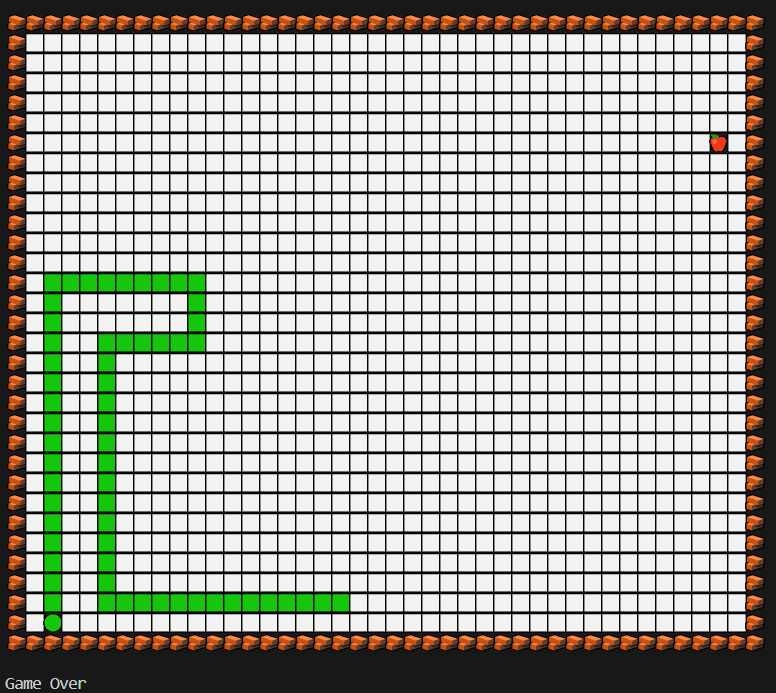
\includegraphics[width=0.6\linewidth]{figures/snakeV1.png}
   \caption{Versión del juego Snake para ordenadores de escritorio}
   \label{figure:snakeV1}
\end{figure}
